%
% Documento: Estrutura
%

\chapter{MATERIAIS E MÉTODOS}

Para o processo de desenvolvimento de sistemas ou aplicativos, antes de mais nada, deve-se realizar o planejamento, etapa onde é formada as ideias, resultando assim, em uma base para os levantamentos dos requisitos, possibilitando uma análise de viabilidade, onde será definido tudo o que será realizável, que por fim tornará possível o fechamento do escopo, originando uma percurso a ser seguido nesse processo.

Nesse contexto, este capítulo apresentará as ferramentas e métodos utilizados para a realização deste trabalho, incluindo os processos de desenvolvimento, bem como as estruturas utilizadas, além das especificações técnicas. A imagem a seguir descreve o fluxo processo de criação utilizado na criação da ferramenta, ilustrando sobre a etapa de planejamento e desenvolvimento

\begin{figure}[H]
    \centering
    \caption{Processo de desenvolvimento}
    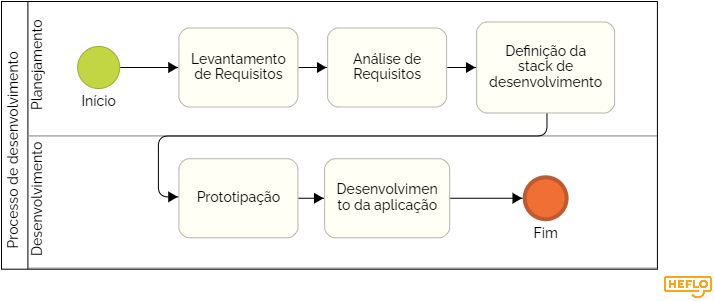
\includegraphics[width=1\textwidth]{figuras/Processo de desenvolvimento Diagrama.png}
    \label{fig:processoDeDesenvolvimento}
    {\fonte{  O Autor (2021).}}
\end{figure}

A Seção \ref{diagramasUML} descreve a modelagem da aplicação assim como a ferramenta utilizada nesse processo. A Seção \ref{wireframes} discorre sobre a etapa de prototipação da interface do sistema e da estratégia utilizada para tanto. E por último, a Seção \ref{ferramentasUtilizadas} transcorre sobre tecnologias que foram utilizadas na criação da ferramenta.


\section{Diagramas UML}
\label{diagramasUML}

A Linguagem de modelagem unificada (UML) foi criada para estabelecer uma linguagem de modelagem visual comum, semanticamente e sintaticamente rica, para arquitetura, design e implementação de sistemas de software complexos, tanto estruturalmente quanto para comportamentos \cite{lucidchart2021}.

A UML usa os pontos fortes destas três abordagens para apresentar uma metodologia mais consistente e mais fácil de usar. Além disso, representa as melhores práticas para desenvolver e documentar aspectos diferentes da modelagem de software e sistemas de negócios \cite{lucidchart2021}.

Como muitos sistemas são concebidos a partir da aplicação de práticas e técnicas de OO, a elaboração de documentos modelando os componentes esperados é feita atualmente a partir de diagramas UML \cite{renatojosegroffe2013}.

Diante deste contexto, foi utilizado no aplicativo para ilustrar as funcionalidades do sistema de cadastro de conteúdo, assim como o funcionamento do aplicativo. A partir disso, foi escolhido o Diagrama de caso de uso para exemplificar a interação entre um ator e o sistema.


\section{Wireframes}
\label{wireframes}

Wireframes são esboços simples de telas de produtos digitais, como sites e aplicativos. O intuito é estruturar e validar ideias, por isso os wireframes não contam com detalhes como cores, fontes, ícones e imagens \cite{editorialaela.io2019}.

Dessa forma, os wireframes conseguem demonstrar de forma direta a arquitetura final de uma interface, posicionando os elementos de forma simples e organizada. Portanto, o wireframe reflete apenas o necessário da proposta de uma interface digital \cite{editorialaela.io2019}.

Contudo, foi utilizado esta ferramenta para criar esboços de telas tanto quanto do sistema de cadastro, onde é possível controlar o conteúdo do mesmo, quanto do aplicativo, contendo todas suas funcionalidades.

\section{Ferramentas Utilizadas}
\label{ferramentasUtilizadas}

Nas seções a seguir são apresentadas as ferramentas de software utilizadas no processo de desenvolvimento do sistema.


\subsection{Figma}
\label{figma}

O Figma é uma ferramenta de design de interface na qual todo o trabalho é feito através do navegador, logo ela é compatível com \textit{Windows}, \textit{Linux}, \textit{Chrome} e \textit{Mac} \cite{siriusinterativa2019}. Essa ferramenta foi utilizada para desenvolver os protótipos em forma de wireframes.

\subsection{Visual Studio Code}
\label{visualStudioCode}

O Visual Studio Code é um editor de código-fonte leve, mas poderoso, que roda em sua área de trabalho e está disponível para \textit{Windows}, \textit{MacOS} e \textit{Linux} \cite{visualstudiocode2021}. Esta ferramenta foi utilizada no desenvolvimento do sistema, possibilitando a codificação do banco de dados, interface e funcionalidades.

\subsection{Insomnia}
\label{insomnia}

O Insomnia é um aplicativo gratuito para desktop que combina uma interface fácil de usar com funcionalidades avançadas, como auxiliares de autenticação , geração de código e variáveis de ambiente \cite{insomnia2021}. Foi utilizado para testes e implementações no banco de dados, também foi utilizado para realizar o gerenciamento de conteúdo.

\subsection{Node.js}
\label{nodejs}

Node.js é uma tecnologia usada para executar código JavaScript fora do navegador. Com ele podemos construir aplicações web em geral, desde websites até APIs e microsserviços \cite{devmedia}. Essa ferramenta foi utilizada no desenvolvimento do banco de dados e do aplicativo.

\subsection{JavaScript}
\label{javaScript}

O JavaScript é uma linguagem leve, interpretada e baseada em objetos com funções de primeira classe, mais conhecida como a linguagem de script para páginas \textit{Web}, mas usada também em vários outros ambientes sem \textit{browser}, tais como node.js,  Apache CouchDB e Adobe Acrobat \cite{mozilla2021}. Essa linguagem foi usada no desenvolvimento do sistema.


\subsection{React Native}
\label{reactNative}

O React Native é um \textit{framework} JavaScript criado para construir a interface do usuário em aplicativos móveis. Baseado no React, o React Native é a solução para criar aplicativos nativos tanto para Android quanto para iOS \cite{devmedia2021}. Essa ferramenta foi utilizada na produção da aplicação \textit{mobile}.

\subsection{Expo}
\label{expo}

Expo é uma estrutura e uma plataforma para aplicações React universais. É um conjunto de ferramentas e serviços criados em torno de plataformas React Native e nativas que ajudam a desenvolver, construir, implantar e iterar rapidamente \cite{expo2021}. Essa ferramenta foi utilizada na produção da aplicação \textit{mobile}.

\subsection{LucidChart}
\label{lucid}

LuicidChart é um aplicativo descrito como uma ferramenta de criação de diagramas inteligentes \cite{Lucid}. Essa ferramenta foi utilizada na elaboração dos diagramas do sistema.

\subsection{Heflo}
\label{heflo}

Heflo é solução BPM para Modelagem e Automatização de Processos de Negócio \cite{Venki}. Essa ferramenta foi utilizada na criação dos diagramas de processos do sistema.



\chapter{Revisão de literatura}
\label{chap:revisaoDeLiteratura}

Neste capítulo serão apresentados conceitos que estão associados ao entendimento e desenvolvimento do presente trabalho. A Seção \ref{engenhariaDeSoftware} irá explicar os principais conceitos da Engenharia de Software assim como sua importância no desenvolvimento de uma aplicação. Já a Seção \ref{tecnologiaMovel} discorrerá sobre as especificações relacionadas à Tecnologia Móvel.

\section{Engenharia de software}
\label{engenhariaDeSoftware}

Segundo \citeonline{pressman2009engenharia}, a Engenharia de Software é a aplicação de uma abordagem sistemática, disciplinada e quantificável no desenvolvimento, na operação e na manutenção de software. Para \citeonline{sommerville_engenharia_2011}, a Engenharia de software tem foco em todos os aspectos da produção de software, desde os estágios iniciais da especificação do sistema até sua manutenção, quando o sistema já está sendo usado. Desse modo, pode-se entender a engenharia como uma série de processos e métodos que possibilitam o gerenciamento e desenvolvimento de software.

Nesse sentido, o presente trabalho fundamenta-se nos preceitos estabelecidos na engenharia de software. Dentre os diversos fundamentos existentes, foram acordados a Engenharia de Requisitos retratado na Seção \ref{engenhariaDeRequisitos} juntamente a Modelagem de Sistemas especificado na Seção \ref{modelagemDeSistemas}.

\subsection{Engenharia de Requisitos}
\label{engenhariaDeRequisitos}

Segundo \citeonline{sommerville_engenharia_2011}, engenharia de requisitos é o processo de descobrir, analisar, documentar e verificar as descrições do que o sistema deve fazer, os serviços que oferece e as restrições a seu funcionamento. Desse modo, pode-se compreender que a Engenharia de Requisitos é responsável por identificar e transformar necessidades dos clientes em algo benéfico, em prol de validar os objetivos de acordo com a finalidade determinada.

Assim sendo, a engenharia de requisitos no presente trabalho tem como objetivo garantir a qualidade final do sistema, através do levantamento dos requisitos de maneira inteligível.

\subsection{Modelagem de Sistemas}
\label{modelagemDeSistemas}

\citeonline{sommerville_engenharia_2011} descreve a modelagem de sistema como processo de desenvolvimento de modelos abstratos de um sistema, em que cada modelo apresenta uma visão ou perspectiva, diferente do sistema. Assim sendo, a Modelagem de Sistemas é responsável por contribuir com a compreensão das funcionalidades por meio de ilustrações.

Dessa forma, o desenvolvimento da solução proposta fundamenta-se nas concepções relacionadas a Engenharia de Software. Assim sendo, a modelagem do sistema proporciona a criação de uma ferramenta que atenda as necessidades das partes interessadas.

\section{Tecnologia Móvel}
\label{tecnologiaMovel}

\citeonline{almeida2011tecnologia} definem a Tecnologia Móvel como a forma de acessar a internet e outros recursos computacionais por meio de dispositivos móveis, tais como, celulares, \textit{iPhone}, \textit{iPod}, \textit{iPad}, \textit{notebooks}, \textit{smart} \textit{pads}, dentre outros.

De acordo com \apudonline{bankmycell}{pessoa2021pesquisa}, os números de utilizadores de \textit{smartphones} têm aumentado exponencialmente ao longo dos anos, verificando-se em 2016 a existência de 2,5 biliões de utilizadores e estimando-se que este número tenha crescido até aos 3,5 bilhões no ano de 2020. 

Desse modo, é possível perceber que a tecnologia móvel tem evoluído cada vez mais ao passar do tempo, criando a oportunidade para o desenvolvimento de diversas ferramentas com diversas funcionalidades. Uma área que pode ser citada dentro das vastas existentes é o \textit{M-Learning} (\textit{mobile learning}), que segundo \citeonline{telefonicaeducaciondigital}, é uma metodologia de ensino que proporciona um novo ambiente para alunos e professores, usando dispositivos móveis como plataformas para viabilizar o aprendizado a distância.

Nesse sentido, a solução proposta, tem o \textit{M-Learning} como um de seus maiores fatores, permitindo o acesso a uma gama de conteúdos de uma forma ágil, possibilitando novos aprendizados ou revisões em curtos períodos de tempo.


\chapter{Trabalhos Correlatos}
\label{chap:trabalhosCorrelatos}

Existem diversos estudos sobre o uso de informática na educação, analisando por completo este cenário, trazendo à tona pesquisas e até mesmo alguns fatos sobre a história da evolução. Dessa maneira, foram feitas buscas por trabalhos para serem utilizados de base que ajudaram no desenvolvimento deste presente trabalho. Dentre estes destacam-se:

\begin{itemize}

\item \textbf{Análise do Projeto de Extensão de Inclusão Digital e Informática Educativa no Ensino Fundamental da Rede Pública}

\citeonline{alves2019analise} abordam em seu trabalho um estudo realizado no projeto de extensão Inclusão Digital e Informática Educativa no Ensino Fundamental da Rede Pública. Desse modo, é feito a contextualização da inclusão digital, das tecnologias de informação e de comunicação (TIC), da informática educativa e por fim da metodologia aplicada ao projeto com o intuito de embasar as pontuações dos resultados da contribuição do uso das tecnologias da informação e comunicação no ensino e nas escolas. Contudo, como resultado eles mostram a importância, benefícios e desafios da informática para crianças do ensino público.

\item \textbf{Crianças e computadores: um estudo exploratório sobre a informática na educação infantil no Distrito Federal}

\citeonline{silva2019crianccas} desenvolve em seu trabalho, uma pesquisa sobre a relação entre crianças e computadores considerando o uso da informática na prática docente dos professores de educação infantil do Distrito Federal. Neste trabalho, é descrito o valor educativo do computador para a educação infantil, os procedimentos metodológicos utilizados durante a realização da pesquisa, e o resultado obtido. Em suma, o trabalho teve como objetivo abordar como os professores da educação infantil utilizam computadores na sala de aula, apontando as dificuldades encontrada pelos mesmos na utilização de tecnologia no ensino.

%\item \textbf{Design de software educacional baseado na teoria dos campos conceituais}

%\begin{citacao}
%Esta dissertação tem como objetivo projetar uma interface educativa a partir do uso de quadro teórico que possibilite a investigação dos significados que emergem durante o uso de um software educacional para ensino de matemática \cite{da2006design}.
%\end{citacao}

\item \textbf{Informática na educação: um olhar sobre a utilização das novas tecnologias no processo de ensino-aprendizagem}

\citeonline{de2017informatica} apresentam em seu trabalho uma visão geral das novas tecnologias da informação e comunicação (TIC) no processo educativo como ferramenta auxiliar na aprendizagem. Dessa forma, é realizado a contextualização entre as inteligências múltiplas e as novas tecnologias e as relaciona, além de detalhar a aplicação da informática no ensino para servir como base do estudo de caso voltado a pesquisa sobre tecnologias na educação. Assim sendo, no trabalho é apontado resultado das pesquisas sobre as escolas que já estão inseridas no mundo tecnológico, também são apresentados os resultados obtidos sobre aspectos positivos e negativos da informática na educação.

\item \textbf{Os Impactos da Informática na Educação Infantil e na Sociedade}

\citeonline{edinaaparecidateixeira2017} disserta em seu trabalho o crescimento tecnológico da informática, as suas influências na sociedade atual e a perspectiva de aplicá-la como instrumento de educação infantil. Em síntese, foi elaborado um levantamento dos fatos relacionados aos impactos da informática na educação infantil e na sociedade, apontando as vantagens da informática no aprendizado de modo geral.

\end{itemize}


\chapter{Aplicativo mobile Computer Instructor}
\label{chap:aplicativoComputerInstructor}
O aplicativo  Computer instructor surgiu a partir da experiência como instrutor no Projeto de Inclusão Digital (PID), onde foi possível perceber que grande parte dos alunos possuíam dúvidas simples que poderiam ser sanadas rapidamente, sem a necessidade da consulta do instrutor, sendo feita uma pesquisa simples e rápida, nesse sentido, foi desenvolvido o sistema com o intuito de remediar essas questões. Dessa forma, a proposta do aplicativo é disponibilizar conceitos e dicas cadastrados pelo professor.

A Seção \ref{coleta} descreve a etapa de coleta e análise de requisitos do sistema, elaborada de acordo com os pontos de carência identificados. Já a Seção \ref{modelagem} irá discorrer sobre a etapa de modelagem através de representações gráficas dos requisitos coletados. A arquitetura do sistema será mostrada na Seção \ref{arquitetura} que explicará a forma em que o sistema foi estruturado. E por último a Seção \ref{implementacao} explana sobre a implementação da ferramenta, mostrando as funcionalidades que foram criadas.

\section{Coleta de requisitos}
\label{coleta}

Coletar os Requisitos é o processo de determinar, documentar e gerenciar as necessidades e requisitos das partes interessadas a fim de cumprir os objetivos \cite{pmbok2017}. Assim sendo, esta etapa é o processo de entendimento e reconhecimento das carências que as partes interessadas esperam ser solucionadas pelo sistema que será desenvolvido, definindo a funcionalidade do sistema.

Por meio da experiência adquirida como instrutor no Projeto de Inclusão Digital da UNIFESSPA, foi feito o levantamento dos requisitos do sistema, com o intuito de auxiliar na aprendizagem do usuário. Dessa forma, foram feitos levantamentos dos requisitos dividindo-os em Funcionais e Não Funcionais.

Segundo \citeonline{sommerville_engenharia_2011}, Requisitos Funcionais podem ser entendidos como serviços que o sistema deve fornecer, de como o sistema deve reagir a entradas específicas e de como o sistema deve se comportar em determinadas situações, já os Requisitos Não Funcionais são restrições aos serviços ou funções oferecidos pelo sistema, muitas vezes, aplicam-se ao sistema como um todo.

A Tabela \ref{tab:requisitos_funcionais} lista os requisitos funcionais coletados. Dentre os requisitos listados, foram implementados na solução proposta deste trabalho todos os requisitos, por serem requisitos desejáveis.


\begin{table}[H]
\centering
\caption{Requisitos Funcionais}
\label{tab:requisitos_funcionais}

\begin{tabular}{|C{0.12\linewidth}|C{0.78\linewidth}|}
\hline
\bfseries ID    & \bfseries Descrição                                           \\ \hline
Req 1 & O professor poderá gerenciar o conteúdo do aplicativo. \\ \hline
Req 2 & O usuário poderá ver informações sobre o aplicativo.   \\ \hline
Req 3 & O usuário poderá acessar módulos dos conteúdos.        \\ \hline
Req 4 & O usuário poderá acessar unidades de cada módulo.      \\ \hline
Req 5 & O usuário poderá acessar o conteúdo de cada unidade.   \\ \hline
\end{tabular}
{\fonte{  O Autor (2021).}}
\end{table}

Os Requisitos Não Funcionais coletados estão relacionados conforme a Tabela \ref{tab:requisitos_funcionais}. Dentre os requisitos listados, foram implementados na solução proposta deste trabalho os requisitos de 1 a 3, por serem requisitos desejáveis, a não implementação do requisito 4 não compromete o funcionamento da ferramenta, já que mesmo sem a interface desenvolvida, ainda é possível realizar o gerenciamento de conteúdo através de outros Apps. A Tabela \ref{tab:requisitos_nao_funcionais} lista os Requisitos Não Funcionais.


\input{tabelas/tabela-requisitos-não-funcionais}

\section{Modelagem de requisitos}
\label{modelagem}

Na linguagem de modelagem unificada (UML), o diagrama de caso de uso resume os detalhes dos usuários do seu sistema (também conhecidos como atores) e as interações deles com o sistema \cite{lucidchart2021uml}. Dentro do contexto do Computer Information, foram criados dois diagramas, o primeiro ilustra o sistema do banco de dados, o segundo demonstra a usabilidade do mesmo.

\subsection{Modelagem back-end}
\label{modelagem_back_end}
Dentro do contexto do backend, existe o seguinte ator:

\begin{itemize}

    \item \textbf{Professor:} É o ator que representa um professor no sistema, ele possui a capacidade de criar, ler, atualizar ou deletar (CRUD) as informações do App.

\end{itemize}

\begin{figure}[H]
    \centering
    \caption{Modelagem do Back-end}
    \includegraphics[width=1\textwidth]{figuras/Backend  Computer Instructor.png}
    \label{fig:modelagemDoBackend}
    {\fonte{ O Autor (2021).}}
\end{figure}

\subsection{Modelagem Computer Instructor}
\label{modelagem_computer_instructor}

Dentro do contexto do  Computer Instructor, existem os seguintes atores:

\begin{itemize}
    \item \textbf{Usuário:} É o ator que representa um usuário do App, ele possui a capacidade de visualizar as informações do App, consultar módulos, as unidades do mesmo, e por fim o conteúdo final contido em cada unidade. Também é possível realizar um filtro através da busca única para módulos e unidades.

    \item \textbf{Professor:} Representa as funções que o sistema disponibiliza para o App, listar módulos e unidades que possuem informações.

\end{itemize}

\begin{figure}[H]
    \centering
    \caption{Computer Instructor - Modelagem}
    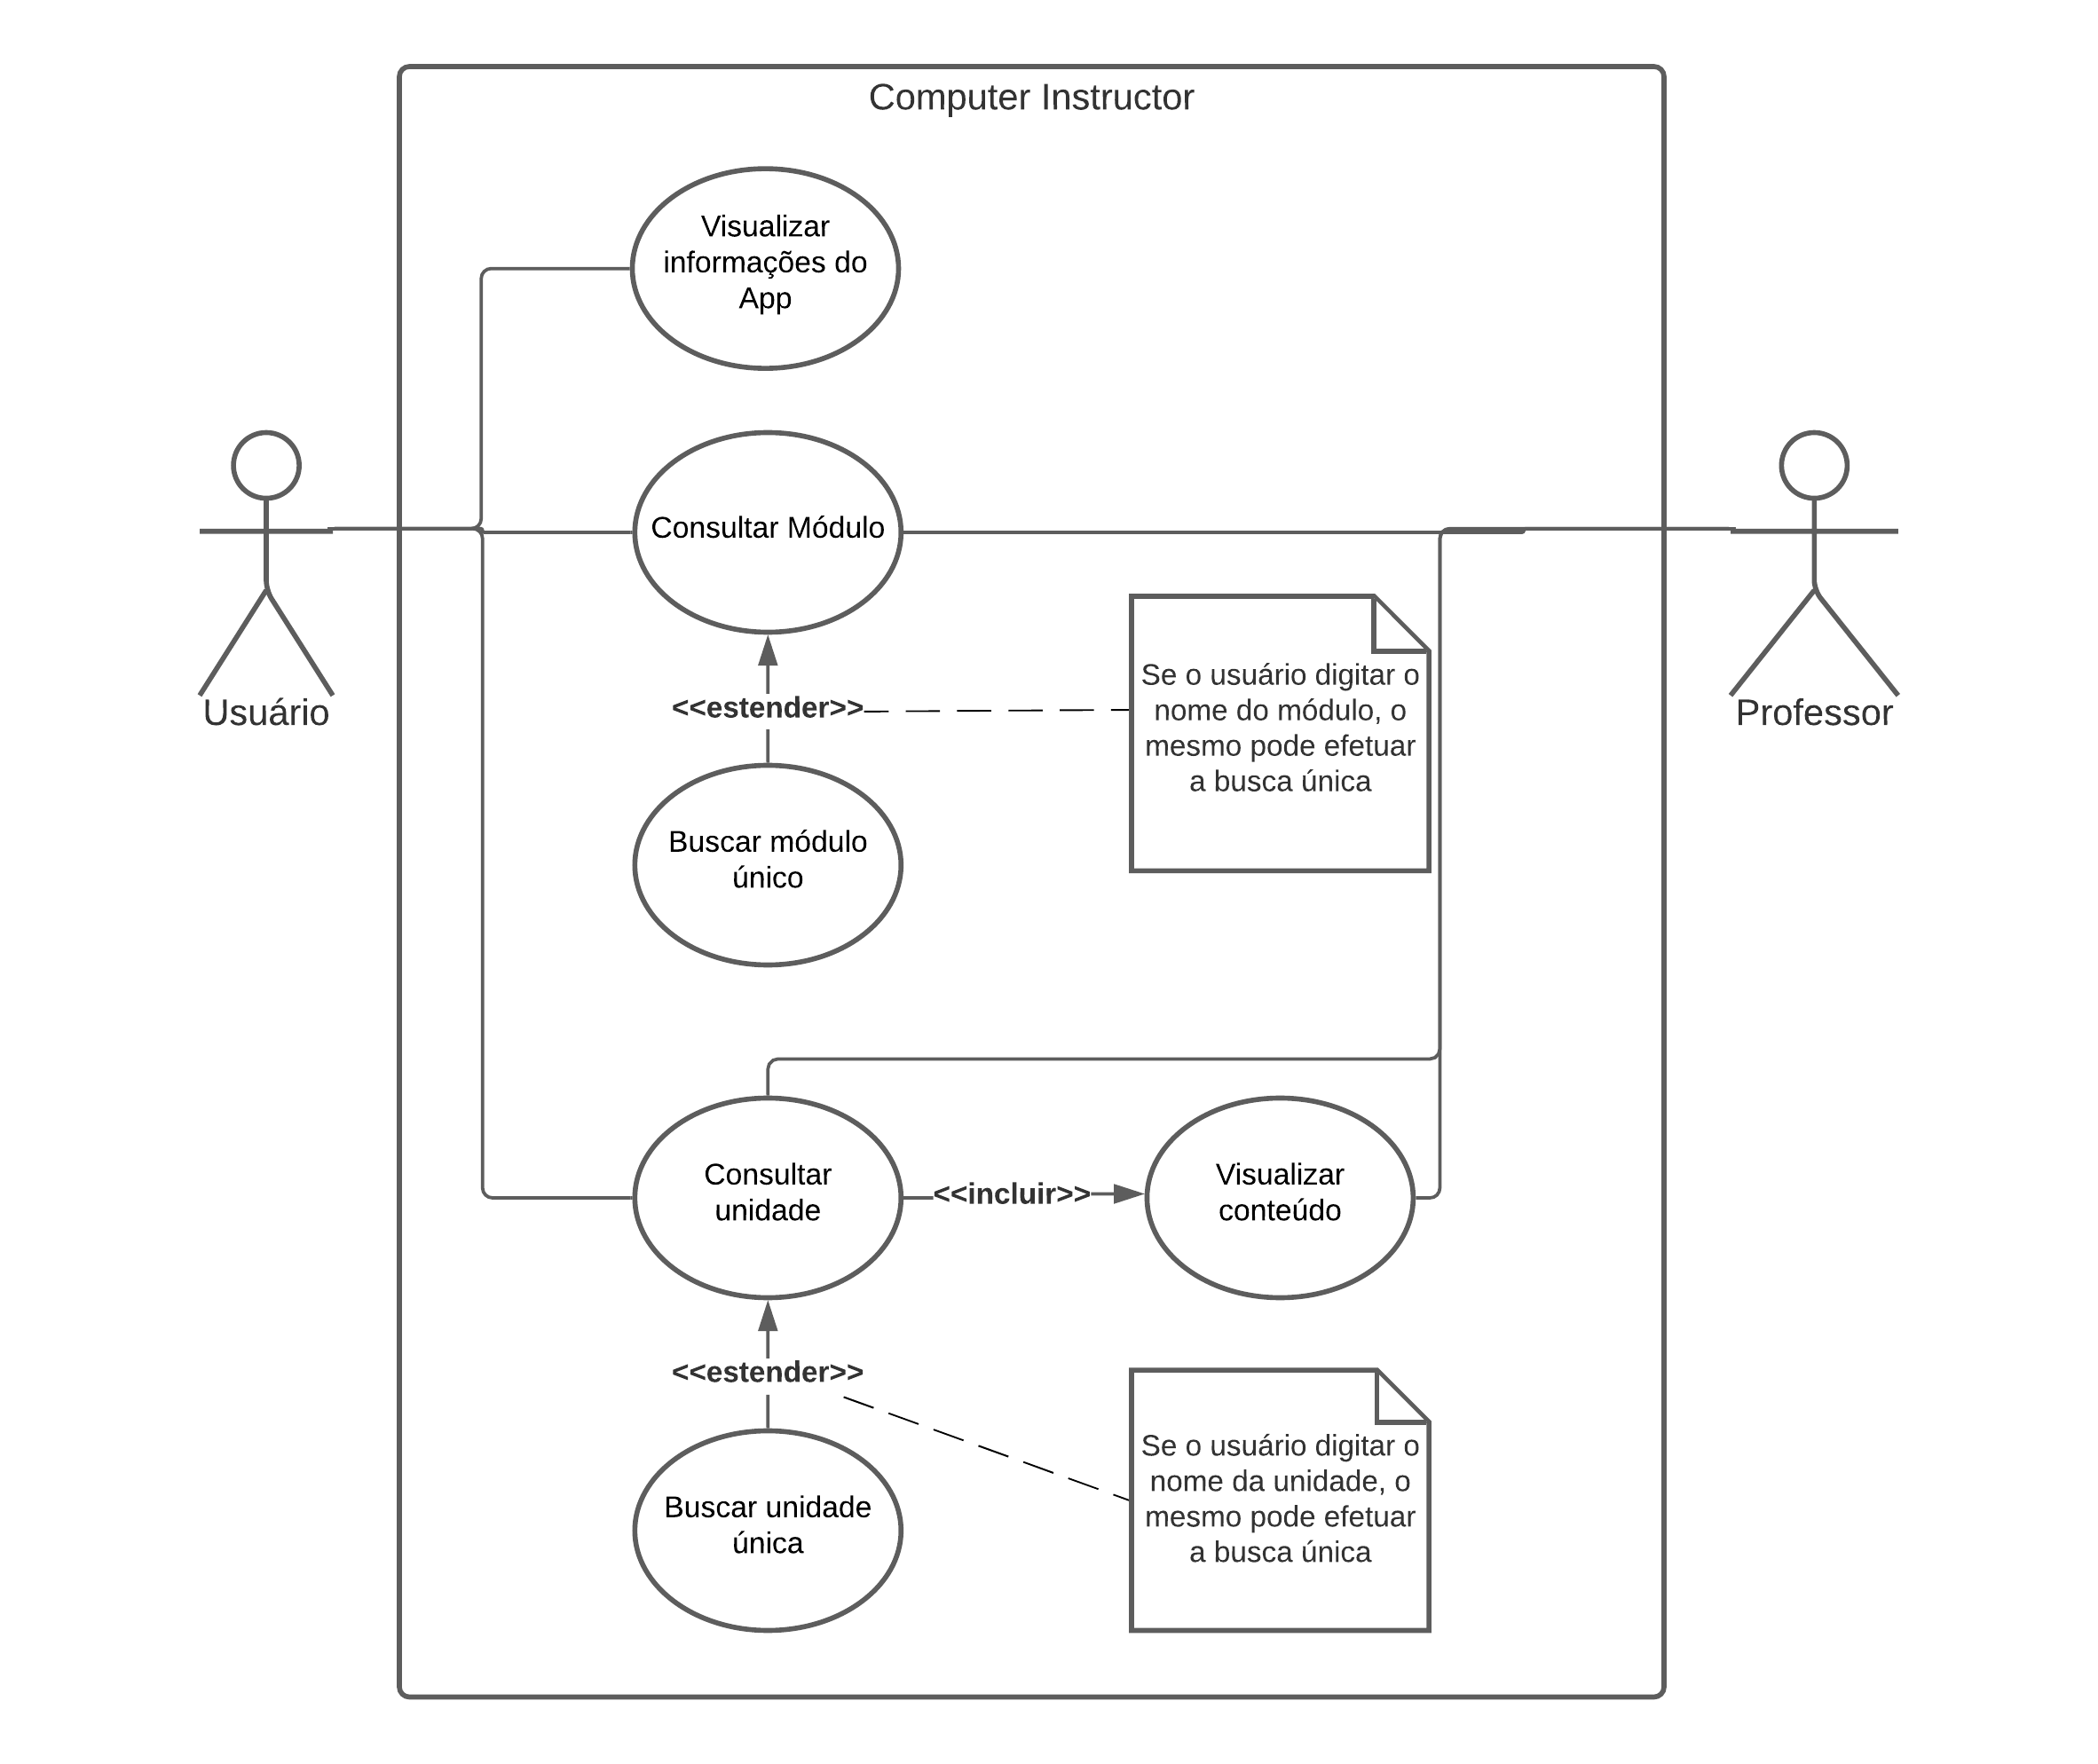
\includegraphics[width=1\textwidth]{figuras/Computer Instructor.png}
    \label{fig:computerInstructor_modelagem}
    {\fonte{ O Autor (2021).}}
\end{figure}

\subsection{Casos de Uso Expandido}
\label{caso_de_uso_expandido}

Os casos de uso também podem ser expandidos textualmente em uma sequência de passos presentes dentro dos mesmos, descrevendo detalhadamente o fluxo do caso de uso. A Tabela \ref{tab:caso_de_uso_extendido} descreve detalhadamente os casos de uso do sistema.


\begin{table}[H]
\centering
\caption{Caso de Uso Expandido}
\label{tab:caso_de_uso_extendido}
\begin{tabular}{|C{0.2\linewidth}|p{0.7\linewidth}|}
\hline

\bfseries Caso de uso:    & \bfseries Gerenciar conteúdo \\ \hline
Ator: & Professor \\ \hline
Fluxo principal: & O professor realiza o gerenciamento do conteúdo usando as quatro operações básicas: CRUD (Create, Read, Update, Delete).   \\ \hline

\bfseries Caso de uso:    & \bfseries Visualizar informações do App \\ \hline
Ator: & Usuário \\ \hline
Fluxo principal: & O usuário visualiza as informações do App, um breve resumo do mesmo.   \\ \hline

\bfseries Caso de uso:    & \bfseries Consultar módulo \\ \hline
Ator: & Usuário \\ \hline
Fluxo principal: & O usuário visualiza os módulos do App e acessa seus conteúdos.   \\ \hline

\bfseries Caso de uso:    & \bfseries Buscar módulo \\ \hline
Ator: & Usuário \\ \hline
Fluxo principal: & O usuário realiza a busca do módulo desejado através da barra de pesquisa.   \\ \hline

\bfseries Caso de uso:    & \bfseries Consultar unidade \\ \hline
Ator: & Usuário \\ \hline
Fluxo principal: & O usuário visualiza as unidades do App e acessa seus conteúdos.   \\ \hline

\bfseries Caso de uso:    & \bfseries Buscar unidade \\ \hline
Ator: & Usuário \\ \hline
Fluxo principal: & O usuário realiza a busca da unidade desejada através da barra de pesquisa.   \\ \hline

\bfseries Caso de uso:    & \bfseries Visualizar conteúdo \\ \hline
Ator: & Usuário \\ \hline
Fluxo principal: & O usuário acessa o conteúdo da unidade desejada.   \\ \hline

\end{tabular}
{\fonte{  O Autor (2021).}}
\end{table}

\subsection{Prototipagem}
\label{prototipagem}
Para auxiliar na síntese das ideias, foi elaborado um esboço das telas através de \textit{Wireframes}, utilizando o Figma para auxiliar este processo. Nas Subsubseções \ref{prototipagem_front} e \ref{prototipagem_mobile} seguem os resultado das prototipações criadas para dar um norte ao projeto.


\subsubsection{Front-end}
\label{prototipagem_front}

O esboço do front-end foi criado para facilitar o gerenciamento do conteúdo do Computer Instructor, possibilitando criar, ler, atualizar ou deletar as informações. Dessa forma, foram divididos 3 componentes para uma melhor experiência do usuário, visando aplicar conceitos de Interação Humano-Computador (IHC), como facilidade do aprendizado, eficiência, facilidade de memorização e satisfação. Assim sendo, segue o resultado da prototipagem ilustrado nas Figuras \ref{fig:wireframe_login}, \ref{fig:wireframe_modulo} e \ref{fig:wireframe_unidade}.

\begin{itemize}
    \item \textbf{Login/Home:}

\begin{figure}[H]
    \centering
    \caption{Wireframe - tela de login}
    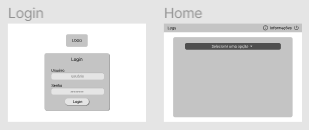
\includegraphics[width=0.8\textwidth]{figuras/Wireframe login-home.png}
    \label{fig:wireframe_login}
    {\fonte{ O Autor (2021).}}
\end{figure}

\item \textbf{Módulo:}


\begin{figure}[H]
    \centering
    \caption{Wireframe - tela de modulos}
    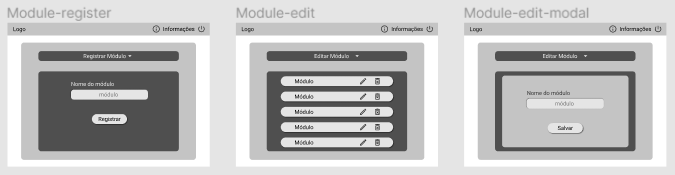
\includegraphics[width=1\textwidth]{figuras/Wireframe modulo.png}
    \label{fig:wireframe_modulo}
    {\fonte{ O Autor (2021).}}
\end{figure}

\item \textbf{Unidade:}


\begin{figure}[H]
    \centering
    \caption{Wireframe - tela de unidades}
    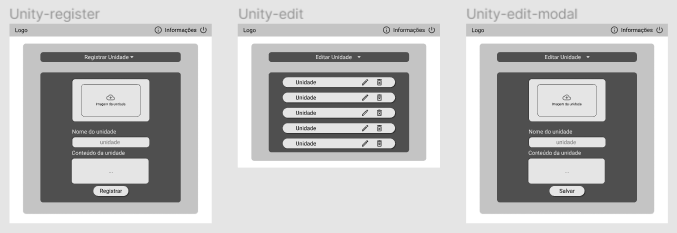
\includegraphics[width=1\textwidth]{figuras/Wireframe unidade.png}
    \label{fig:wireframe_unidade}
    {\fonte{ O Autor (2021).}}
\end{figure}

\end{itemize}

\subsubsection{Mobile}
\label{prototipagem_mobile}

O esboço do App foi criado visando a simplicidade, implementando os requisitos para proporcionar agilidade e facilidade no aprendizado do usuário. Nesse sentido, foi desenvolvido a prototipagem do Computer Instructor em forma de \textit{wireframes}. Dessa forma, a Figura \ref{fig:wireframe_mobile} mostra o resultado da prototipagem.

\begin{figure}[H]
    \centering
    \caption{Wireframes - Mobile}
    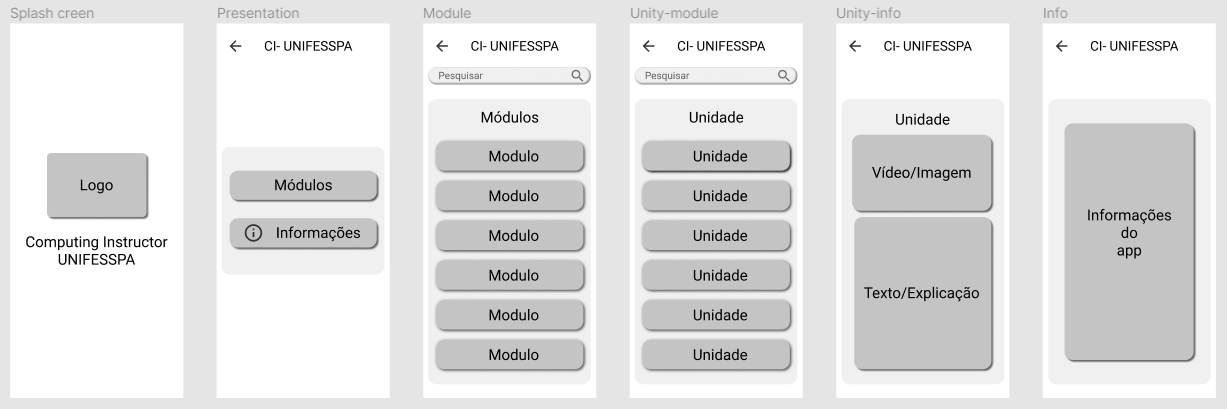
\includegraphics[width=1\textwidth]{figuras/Wireframe mobile.png}
    \label{fig:wireframe_mobile}
    {\fonte{  O Autor (2021).}}
\end{figure}

\section{Arquitetura do  Computer Instructor}
\label{arquitetura}

A Figura \ref{fig:arquitetura_backend} mostra a arquitetura que foi utilizada na criação do aplicativo  Computer Instructor. O Banco de Dados é responsável por guardar as informações do sistema, como os módulos, suas unidades e seus conteúdos, já o Armazenamento de Arquivos tem o intuito de armazenar as mídias cadastradas no App, sendo estes vídeos ou imagens, e todo o controle do conteúdo é feito pelo professor diretamente no Backend.

\begin{figure}[H]
    \centering
    \caption{Backend Computer Intructor}
    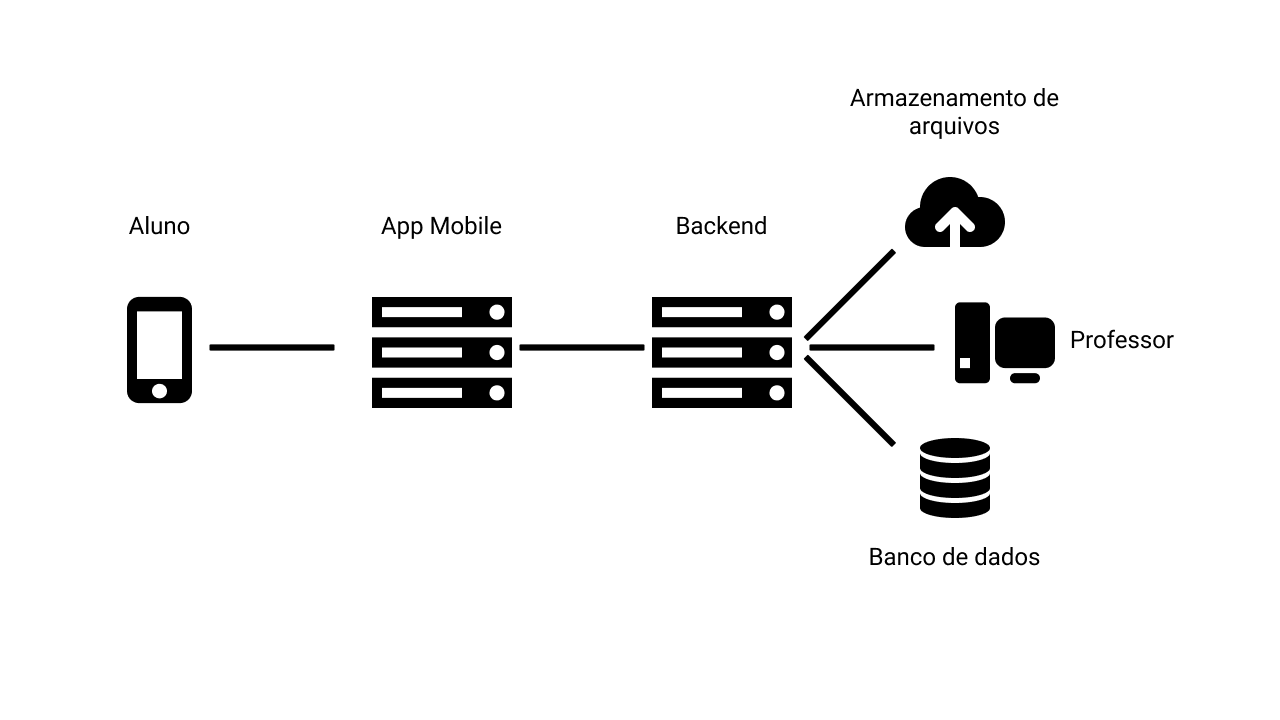
\includegraphics[width=1\textwidth]{figuras/Arquitetura - Computer Instructor.png}
    \label{fig:arquitetura_backend}
    {\fonte{  O Autor (2021).}}
\end{figure}

O Back-end vem da ideia do que tem por trás de uma aplicação \cite{mariosouto2019}. Dessa forma, funciona como uma API (\textit{Application Programming Interface}), um conjunto de funções estabelecidas por um software, que funcionam como uma interface intermediária, para a utilização de funcionalidades deste software por aplicações externas \cite{andersonirias2019}.

O Mobile por sua vez, se trata de um software desenvolvido para ser instalado em \textit{smartphones} e \textit{iPads}. Como pode ser visto na figura anterior o App não possui interação com o Banco de Dados ou o Armazenamento de Arquivos, pois todo gerenciamento é feito pelo professor, adicionando, alterando ou removendo os conteúdos através da API, o que garante que as informações gerenciadas passem pelo Back-end que é onde estão as regras de negócio, isso garante que o sistema possua integridade nos dados armazenados.
Os Alunos acessam o sistema através do App mobile, utilizando a interface provida. Dessa forma, não há interação direta dos alunos com o Back-end, Banco de Dados ou Armazenamento de Arquivos.

A estratégia de divisão das responsabilidades do sistema entre o Back-end e o Front-end é utilizada para garantir uma melhor manutenabilidade, separando a parte lógica, onde ocorre o processamento dos dados, da interface gráfica do sistema, a parte usual, onde é possível interagir com uma aplicação. Além disso, também foi utilizado a estratégia da utilização de um sistema de banco de dados separado do armazenamento de arquivos com o intuito de conseguir um melhor desempenho do banco de dados da aplicação, por não precisar manipular arquivos extensos.


\section{Implementação do  Computer Instructor}
\label{implementacao}

A implementação da aplicação foi feita utilizando a linguagem de programação Javascript tanto no Back-end quanto no App mobile, que por sua vez foi desenvolvido utilizando como base o \textit{framework} React Native. O desenvolvimento da interface foi feito idealizando uma solução que fosse funcional, amigável e minimalista, seguindo o conceito \textit{Affordance}, que segundo \citeonline{homemmaquina2014},  é o potencial de um objeto de ser usado como foi projetado para ser usado. Nas Subseções \ref{implementacao_back} e \ref{implementacao_mobile} serão descritos as criações do Back-end e do aplicativo Mobile, respectivamente. 

\subsection{Back-end}
\label{implementacao_back}

O Back-end da aplicação foi desenvolvido utilizando a linguagem de programação Javascript, utilizando o modelo REST (\textit{REpresentational State Transfer}), que representa nada mais que uma “nova” possibilidade para a criação de \textit{web services}, utilizando a semântica dos métodos HTTP (\textit{GET}, \textit{POST}, \textit{PUT} e \textit{DELETE}), na leveza dos pacotes de dados transmitidos na rede e na simplicidade, o que torna desnecessária a criação de camadas intermediárias \cite{devmedia2018}. Dessa forma o Back-end da aplicação é responsável por dispor as funções através das rotas presentes nele, desempenhando o papel de ser a parte lógica do sistema, operando a base de dados e com o armazenamento de arquivos.

A Figura \ref{fig:diagram_entidade_relacionamento} mostra como as entidades se relacionam entre si dentro do sistema, através de um diagrama entidade-relacionamento (ER). Na imagem é possível perceber que o banco de dados é constituído de duas entidades, uma chamada \textit{module}, que consiste em representar os módulos que possuem unidades, outra entidade, denominada \textit{unity}, cuja mesma engloba o conteúdo final do App.

\begin{figure}[H]
    \centering
    \caption{Diagrama Entidade-relacionamento}
    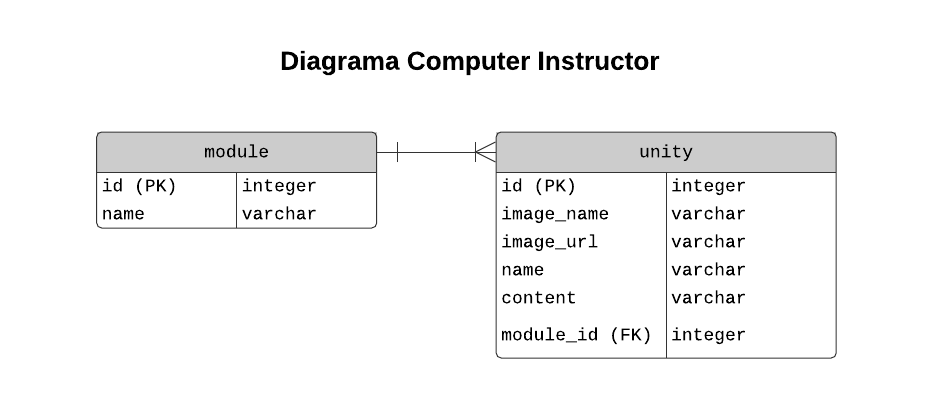
\includegraphics[width=1\textwidth]{figuras/Diagrama ER.png}
    \label{fig:diagram_entidade_relacionamento}
    {\fonte{  O Autor (2021).}}
\end{figure}

\subsection{Mobile}
\label{implementacao_mobile}
O aplicativo mobile foi desenvolvido utilizando a linguagem de programação Javascript, utilizando o \textit{framework} React Native, com o intuito de escrever um único código para funcionar tanto no Android quanto no iOS de forma nativa, criando assim um App multiplataforma.

A figura \ref{fig:wireframe_mobile_tela_inicial} mostra a tela inicial da aplicação, onde de maneira objetiva, há a opção de ver o conteúdo, ou informações sobre a criação do mesmo.

\begin{figure}[H]
    \centering
    \caption{Mobile - Página incial}
    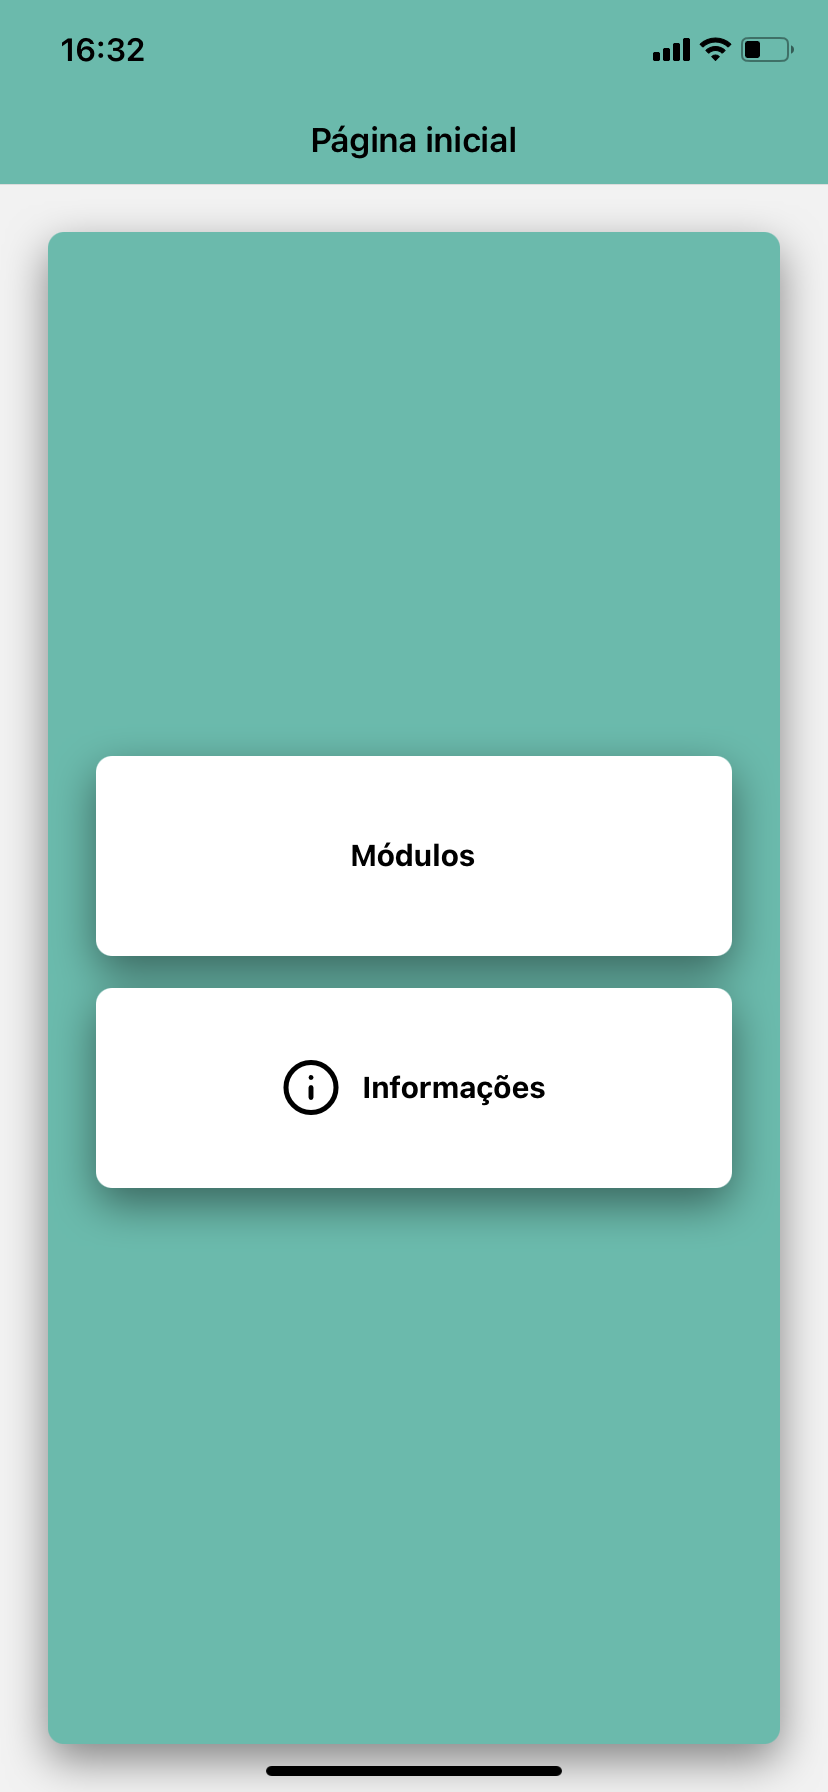
\includegraphics[width=0.5\textwidth]{figuras/Mobile - pagina inicial.png}
    \label{fig:wireframe_mobile_tela_inicial}
    {\fonte{  O Autor (2021).}}
\end{figure}

Na figura \ref{fig:wireframe_mobile_tela_de_informacoes} pode-se ver a tela de informações, onde contém de forma sucinta o propósito e o objetivo do aplicativo.

\begin{figure}[H]
    \centering
    \caption{Mobile - Página de informações}
    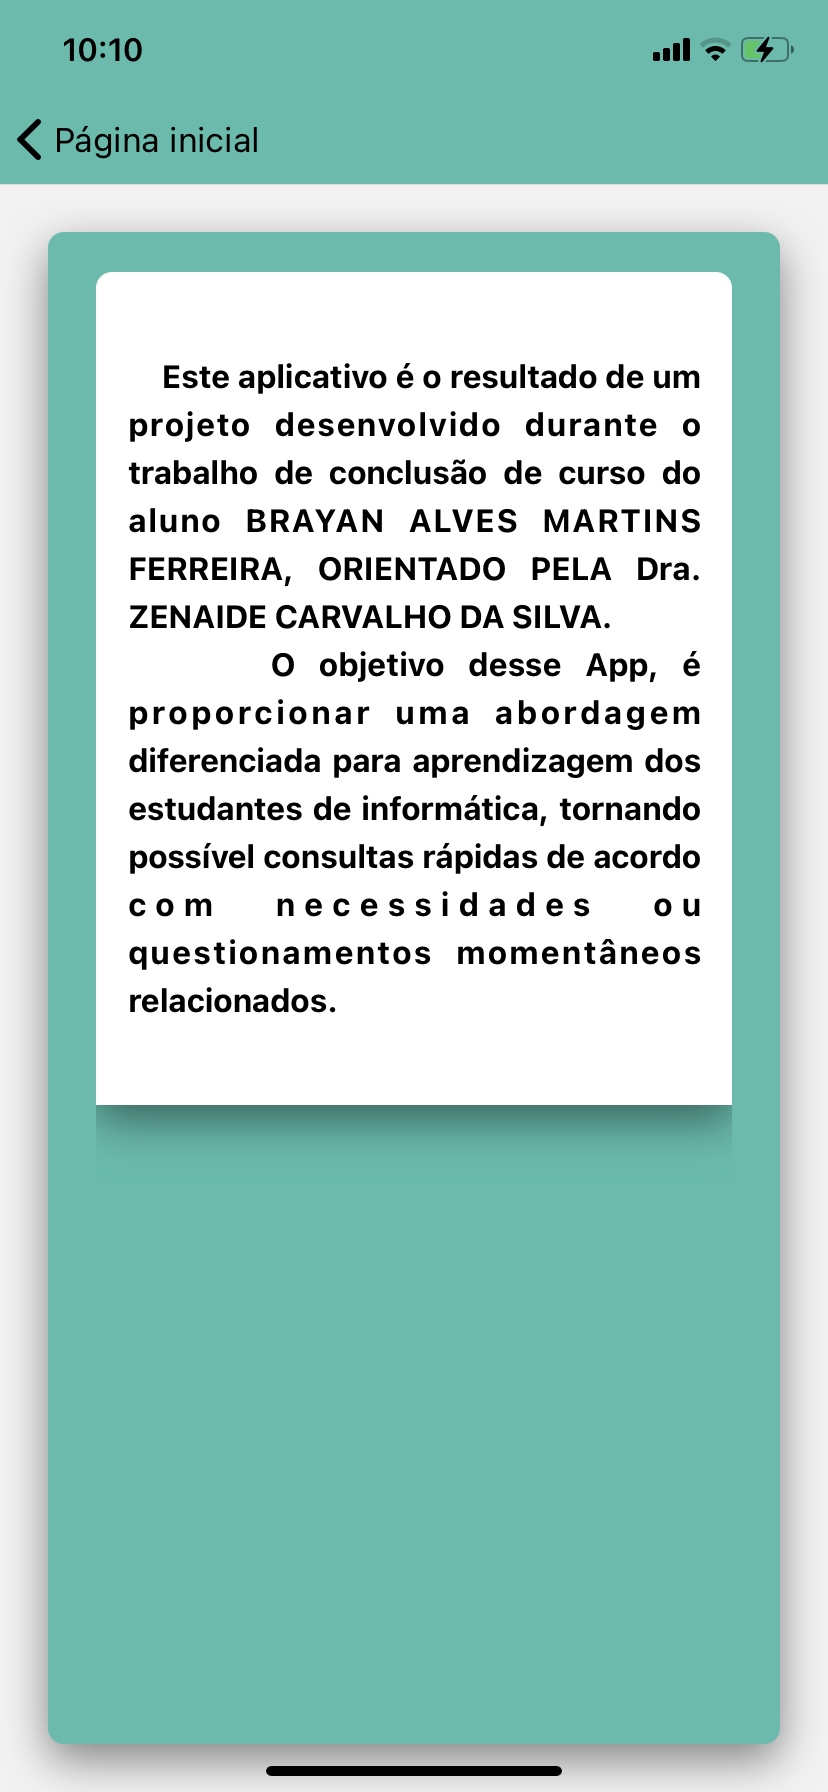
\includegraphics[width=0.5\textwidth]{figuras/Mobile - pagina de informacoes.png}
    \label{fig:wireframe_mobile_tela_de_informacoes}
    {\fonte{  O Autor (2021).}}
\end{figure}

Na Figura \ref{fig:wireframe_mobile_tela_de_modulos} pode-se ver a tela dos módulos que dividem os conteúdos do aplicativo, também é possível efetuar um filtro para encontrar de maneira mais ágil o módulo desejado. Cada módulo pode conter várias unidades, proporcionando uma diversidade de conteúdo.

\begin{figure}[H]
    \centering
    \caption{Mobile - Página de módulos}
    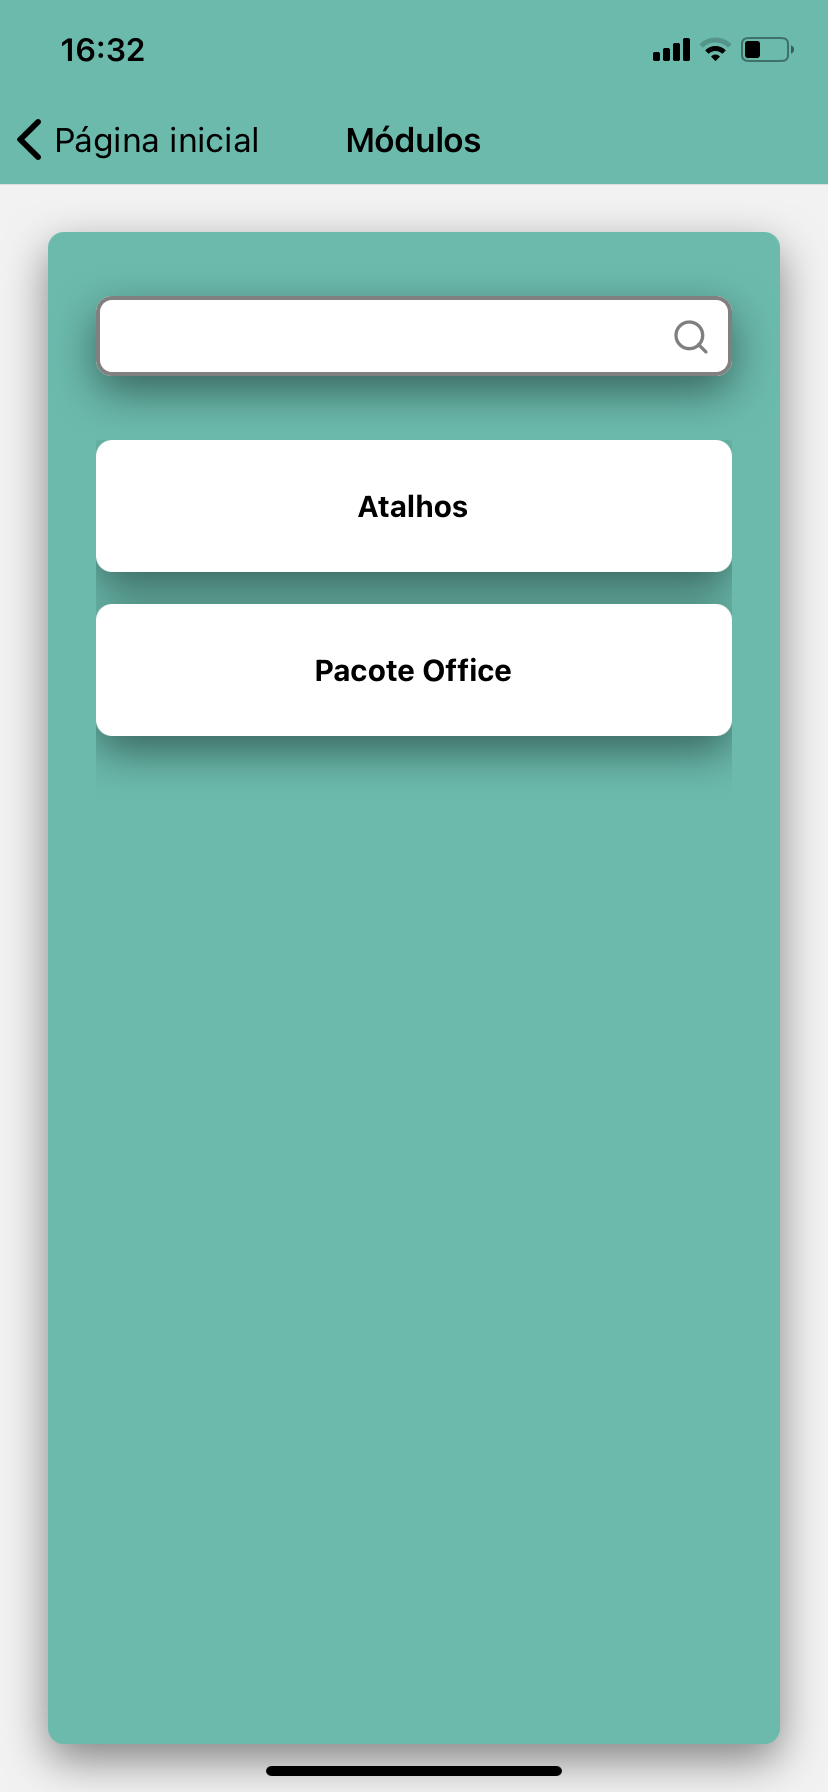
\includegraphics[width=0.5\textwidth]{figuras/Mobile - modulos.png}
    \label{fig:wireframe_mobile_tela_de_modulos}
    {\fonte{  O Autor (2021).}}
\end{figure}

As Figuras \ref{fig:wireframe_mobile_tela_de_unidades} e \ref{fig:wireframe_mobile_tela_de_unidades2} mostram as telas relacionadas às unidades de cada módulo, ilustrando 2 exemplos de diferentes unidades contidas no mesmo, onde cada um possui conteúdo, também é possível efetuar um filtro para encontrar de maneira mais ágil a unidade desejada.

\begin{figure}[H]
    \centering
    \caption{Mobile - Página de unidades}
    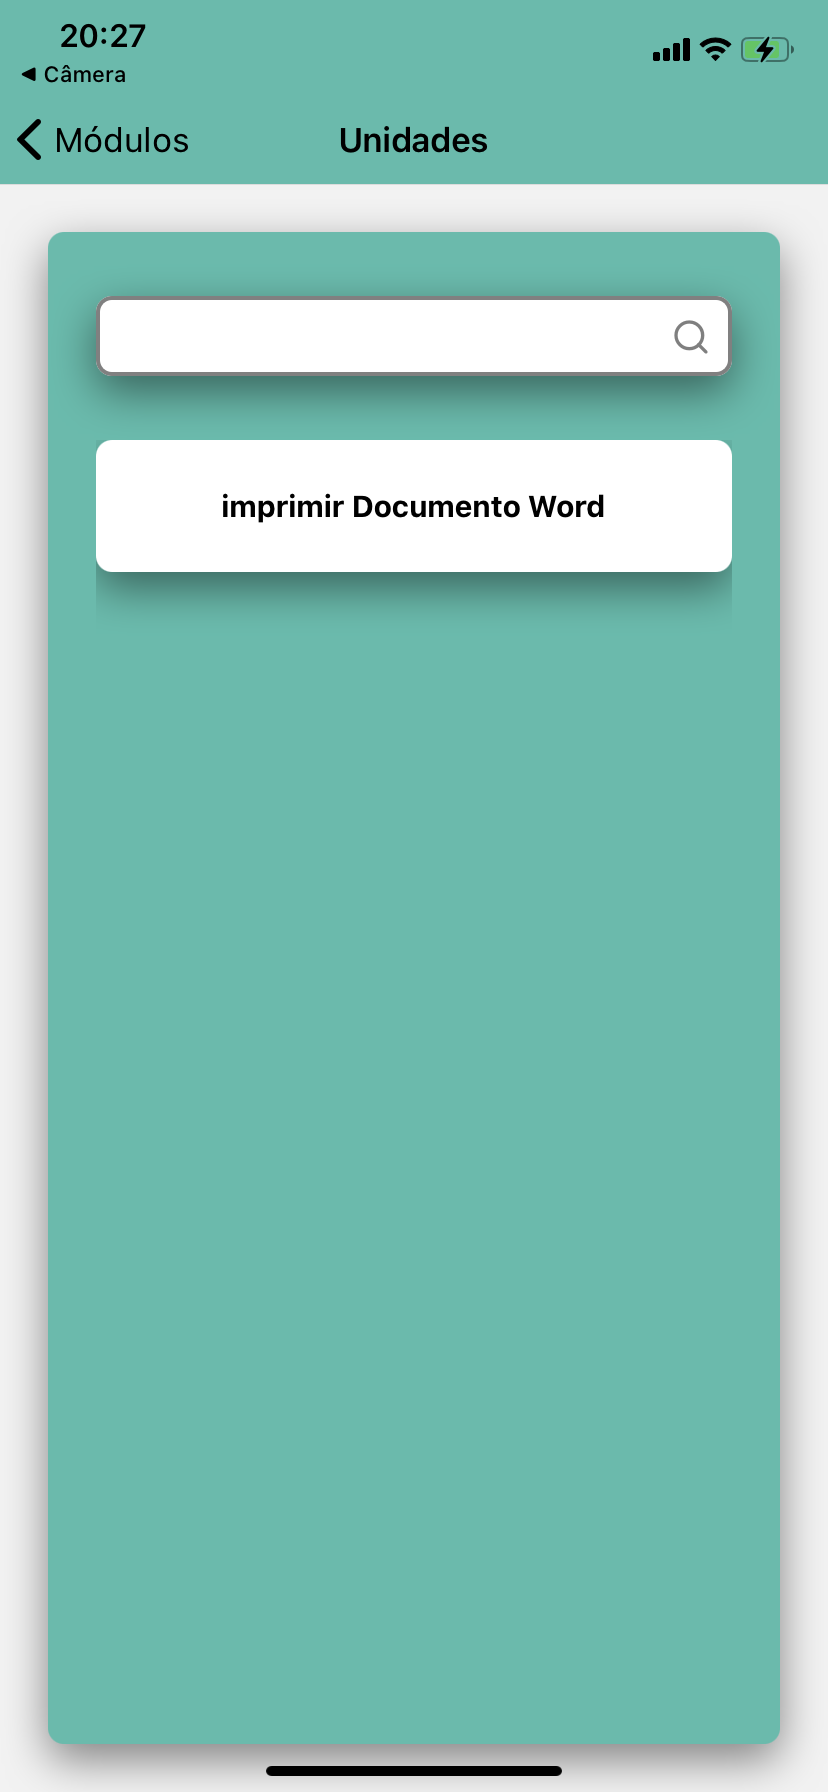
\includegraphics[width=0.5\textwidth]{figuras/Mobile - pagina de unidade.PNG}
    \label{fig:wireframe_mobile_tela_de_unidades}
    {\fonte{  O Autor (2021).}}
\end{figure}

\begin{figure}[H]
    \centering
    \caption{Mobile - Página de unidades 2}
    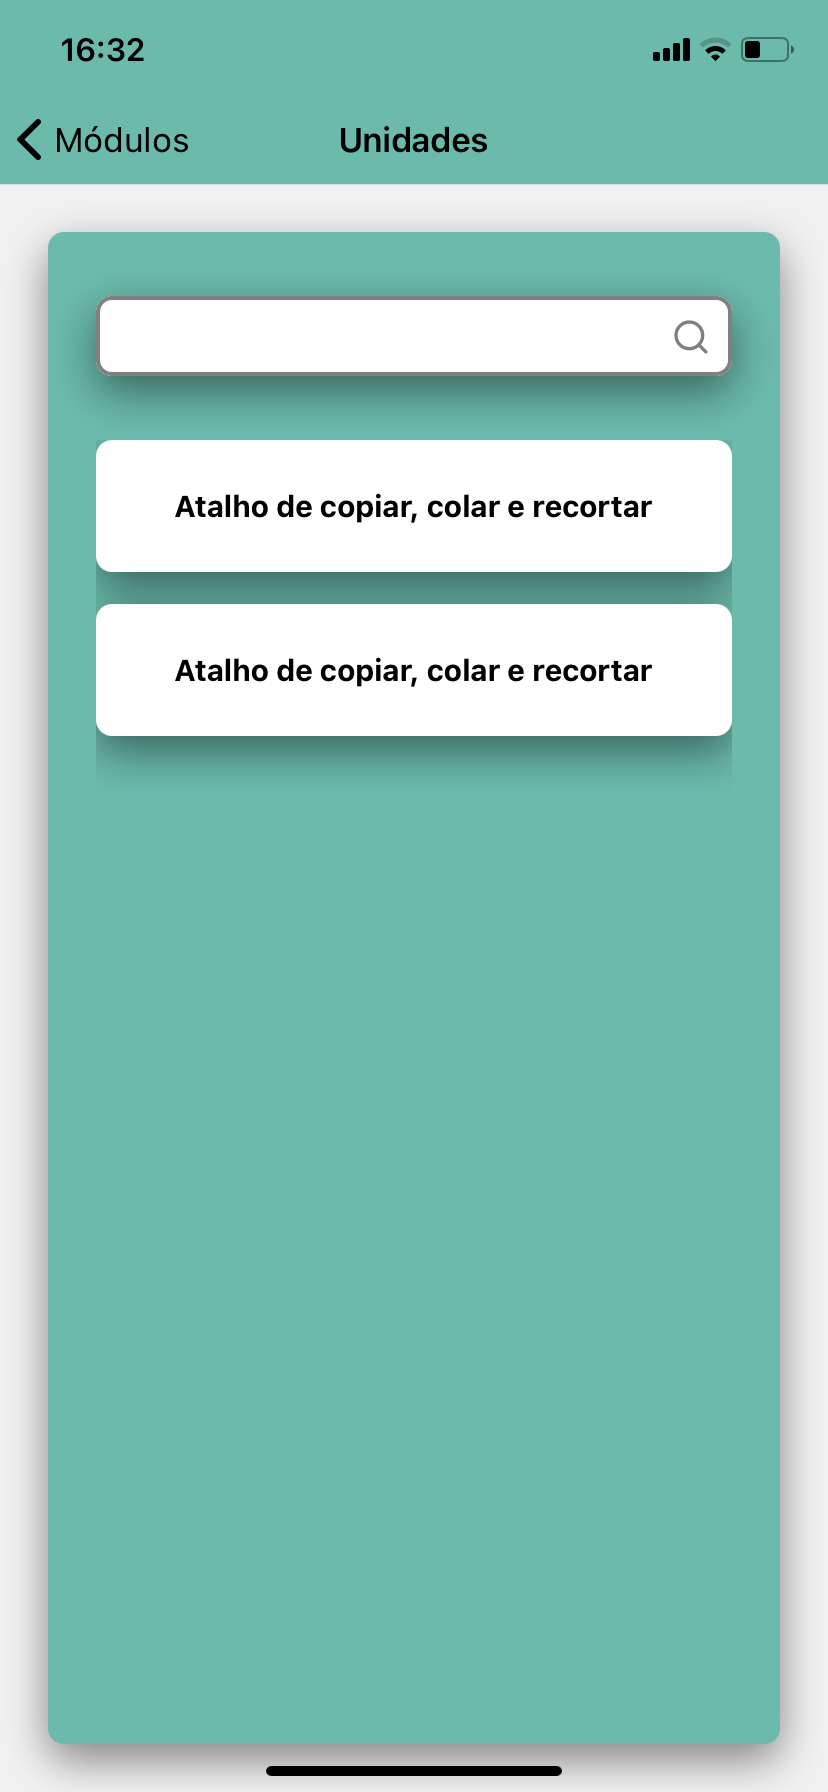
\includegraphics[width=0.5\textwidth]{figuras/Mobile - pagina de unidade2.png}
    \label{fig:wireframe_mobile_tela_de_unidades2}
    {\fonte{  O Autor (2021).}}
\end{figure}

Nas Figuras \ref{fig:wireframe_mobile_tela_de_conteudo}, \ref{fig:wireframe_mobile_tela_de_conteudo2} e \ref{fig:wireframe_mobile_tela_de_conteudo3} é ilustrado a tela final, onde contém o conteúdo final de cada unidade, na mesma é possível ver além de uma explicação textual, uma ilustração em mídia, seja em imagem, gif, ou até mesmo vídeo, com o intuito de ser bem simples e objetivo, tornando-o prático.

\begin{figure}[H]
    \centering
    \caption{Mobile - Página de conteúdo}
    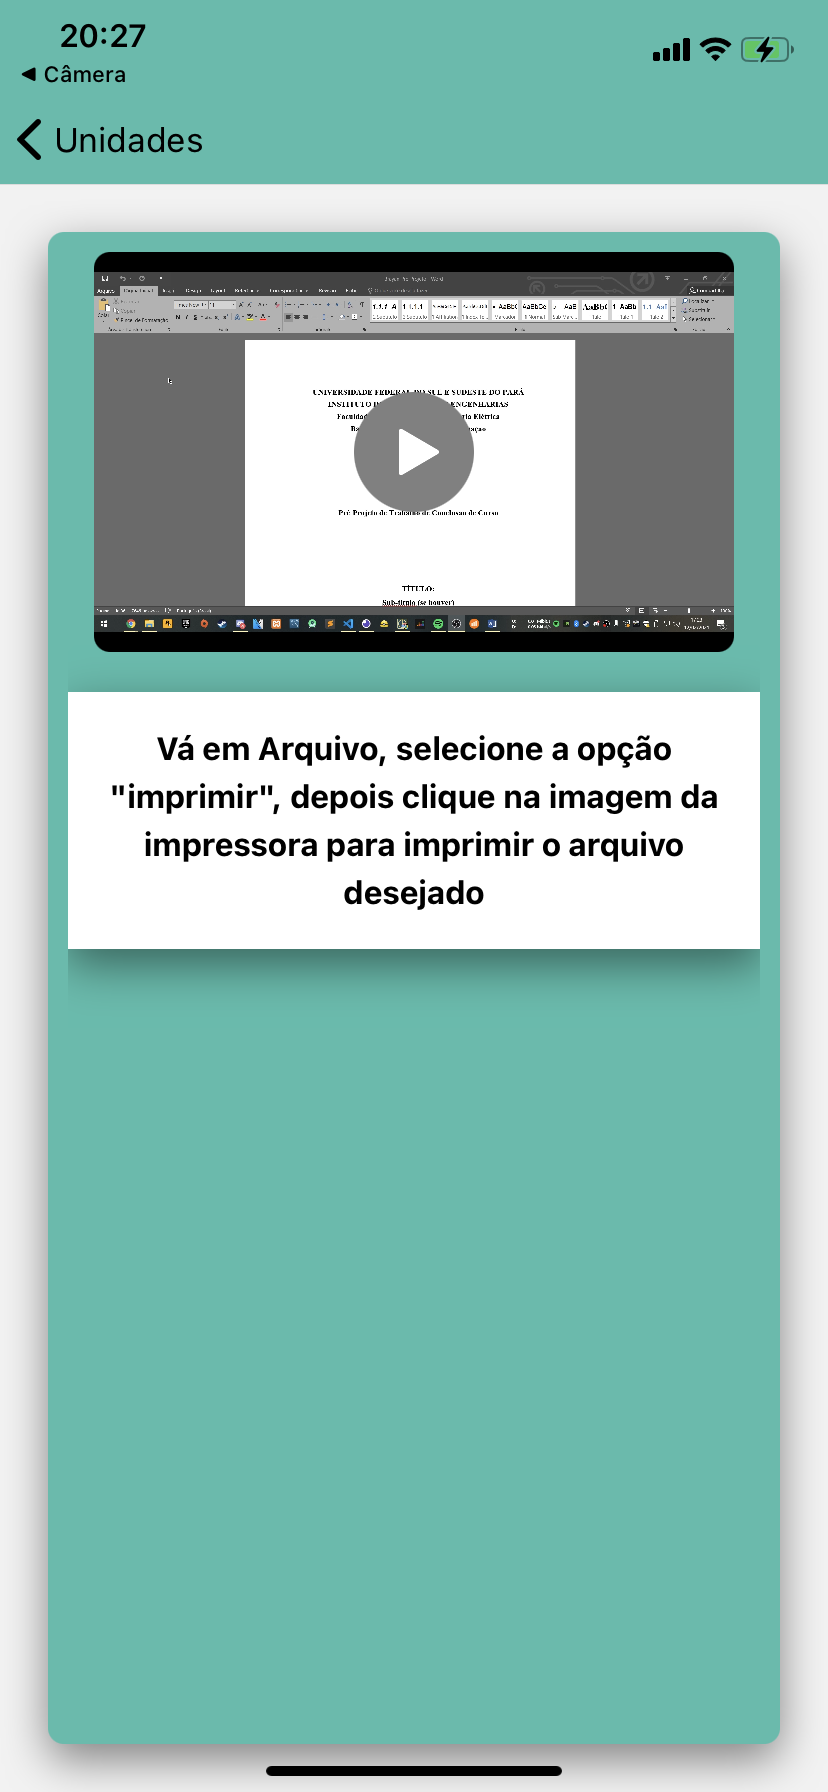
\includegraphics[width=0.5\textwidth]{figuras/Mobile - pagina de conteudo.png}
    \label{fig:wireframe_mobile_tela_de_conteudo}
    {\fonte{  O Autor (2021).}}
\end{figure}

\begin{figure}[H]
    \centering
    \caption{Mobile - Página de conteúdo 2 }
    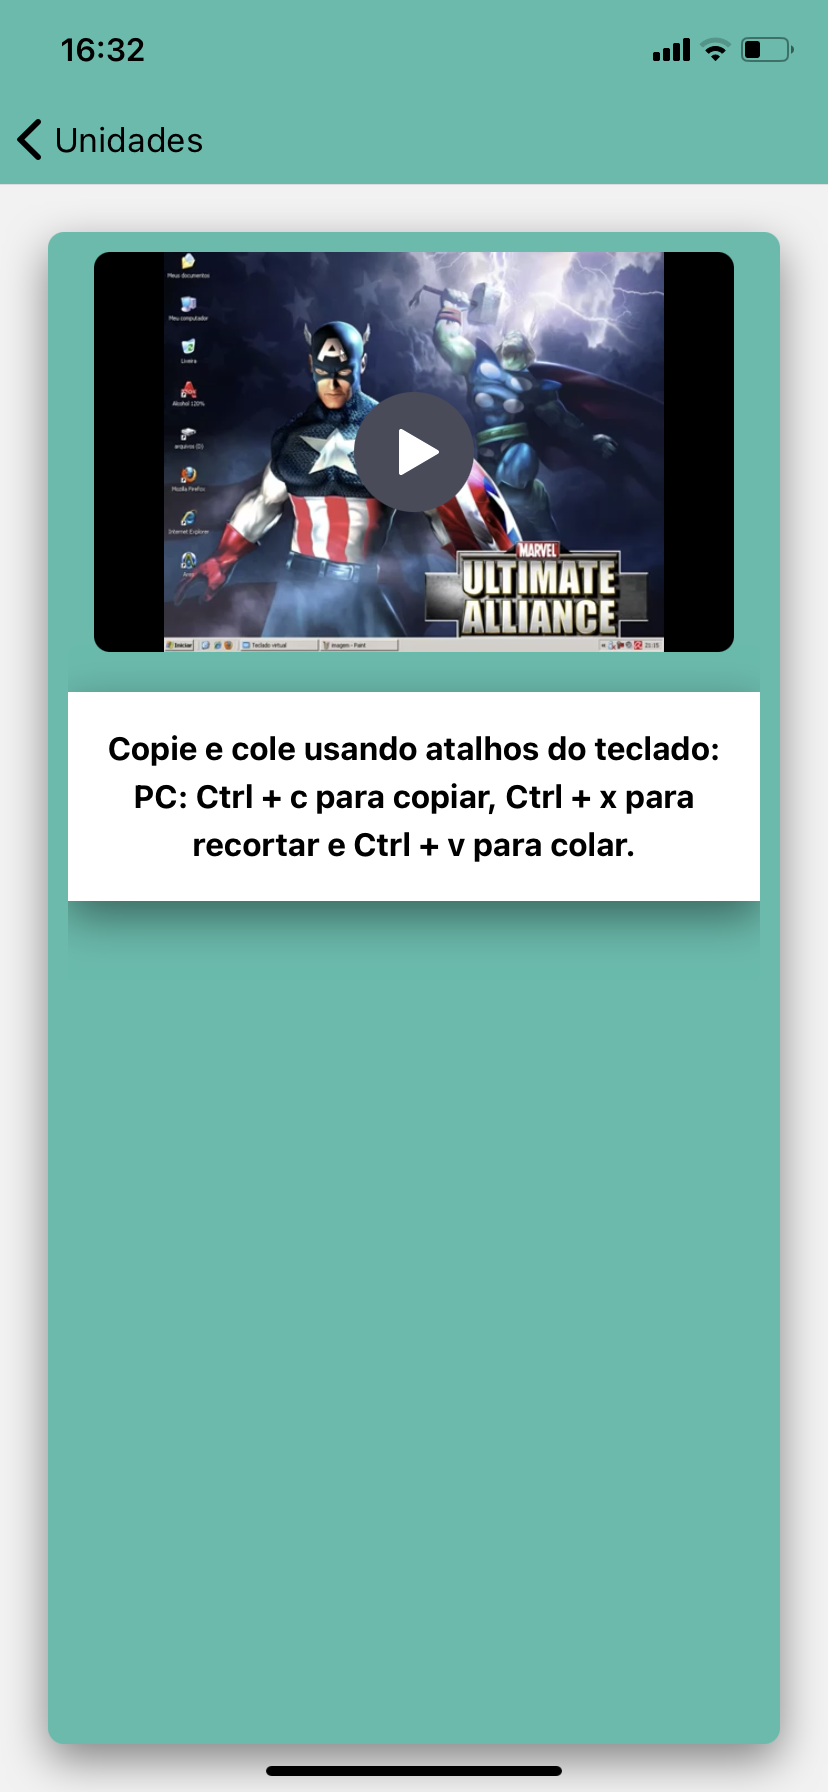
\includegraphics[width=0.5\textwidth]{figuras/Mobile - pagina de conteudo2.png}
    \label{fig:wireframe_mobile_tela_de_conteudo2}
    {\fonte{  O Autor (2021).}}
\end{figure}

\begin{figure}[H]
    \centering
    \caption{Mobile - Página de conteúdo 3}
    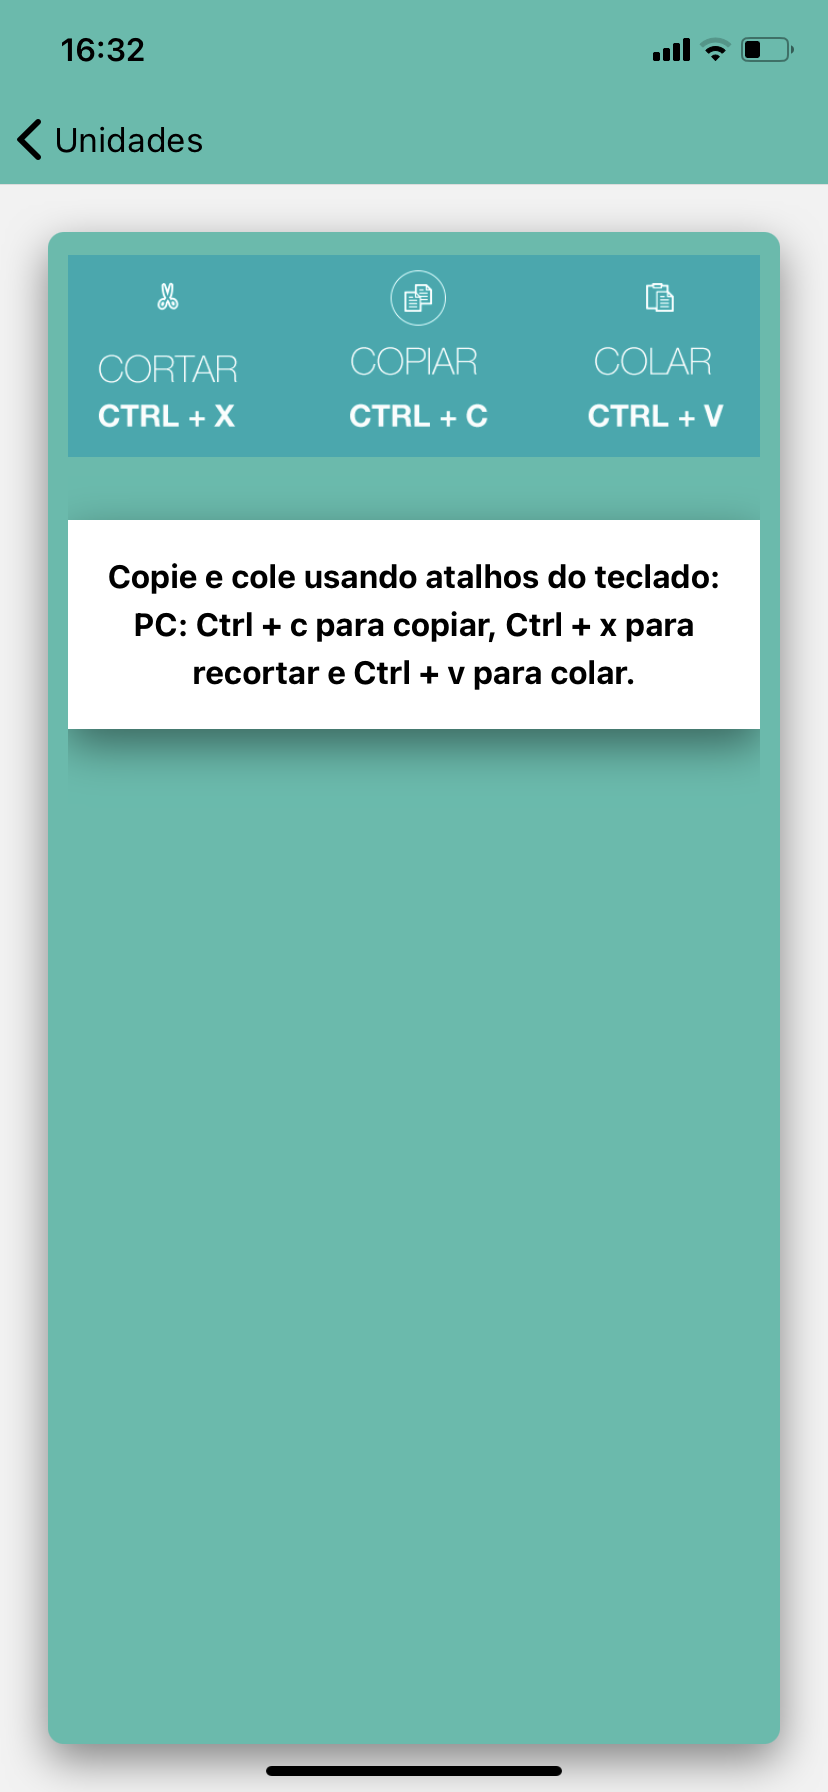
\includegraphics[width=0.5\textwidth]{figuras/Mobile - pagina de conteudo3.png}
    \label{fig:wireframe_mobile_tela_de_conteudo3}
    {\fonte{  O Autor (2021).}}
\end{figure}